\documentclass[8pt, oneside]{article}   	
\usepackage[top=1in, bottom=1in, left=1in, right=1in]{geometry} 		
\geometry{letterpaper}                   		

\usepackage{hyperref}
\usepackage{graphicx}												
\usepackage{amssymb}
\usepackage{array,multirow,graphicx}
 \usepackage{float}
 \usepackage{rotating}
 \usepackage{adjustbox}

\title{Pakistan Poverty Estimation}

\begin{document}

\maketitle

\section{Introduction}

Understanding which households are poor and which households experience worsening poverty levels over time is important in effectively targeting resources. However, poverty surveys can be expensive and time consuming. This project will test the feasibility of using publicly and freely available data to identify poor households and identify which households experienced worsening poverty over time. In particular, we rely on satellite imagery, facebook usage data, among other sources for poverty prediction.\footnote{This work builds on an existing literature that uses satellite data, facebook data and other nontraditional data sources for poverty estimation. For example, see \href{https://web.stanford.edu/~mburke/papers/JeanBurkeEtAl2016.pdf}{Jean et al (2016)}, \href{https://www.itu.int/dms_pub/itu-s/opb/journal/S-JOURNAL-ICTF.VOL1-2018-2-P04-PDF-E.pdf}{Weber et al (2018)}}.
\par
Poverty estimates derived from nontraditional data sources are not a substitute for household surveys. Surveys are needed to train algorithms and surveys capture a wider breadth of characteristics than nontraditional data sources are able to. However, nontraditional data sources can supplement surveys by allowing for poverty estimates in years without a survey and can identify areas that likely saw notable decreases in poverty levels, alerting officials to follow up with these select areas.

\section{Data Sources}

We rely on four rounds of survey data from the Benazir Income Support Project (BISP) for poverty data, surveyed in 2011, 2013, 2014 and 2016. Roughly 8,000-9,000 households were surveyed each year across Pakistan; however, geographic coordinates were only recorded in 2011 and 2013 and within these years only about half the households had coordinates recorded (see \autoref{tab:bisp_sum_stat}). For households that were resurveyed in 2014 and 2016 we rely on the geographic coordinates of the households in 2011 and 2013. Average poverty scores and the proportion of households considered poor are roughly the same between the full sample of households and the sample with coordinates for all years except 2016.
\par
We rely on four sources of publicly available data to predict poverty levels:
\begin{itemize}
\item {\bf Nighttime Lights:} We use nighttime lights data from the Visible Imaging Radiometer Suite (VIIRS) onboard the Suomi National Polar-orbiting Partnership satellite. VIIRS provides nighttime lights values for 750 meter pixels from April 2012 to the present. We extract monthly averages and create a number of metrics at the annual level, including average, minimum, maximum and standard deviation of nighttime lights across months in a year within areas 1, 2, 5 and 10km from each household. 
\item {\bf Daytime Imagery:} We use daytime imagery from landsat which is available from the 1980s to the present. Imagery is available at a 30 meter resolution roughly every two weeks. Landsat data contains seven bands, representing different reflectance along the electromagnetic spectrum (e.g., reflectance of visible light -- red, green and blue, and othe bands such as infrared). The individual bands themselves do not provide an intuitive meaning; however, combinations of bands provide an intutitive meaning. For example, combining red and infrared bands provides a measure of the amount of vegetation.
\item {\bf Facebook Useage:} We scrape data on daily and monthly active users on Facebook using Facebook's marketing API. The marketing API allows determining the number of facebook users by characteristics---for example, the number of male or female users, the number of users with a select educational background, or the type of phone (e.g., high end or cheap) used to access Facebook. 
\item {\bf Open Street Maps:} We integrate road data from Open Street Map, measuring the distance of households to the nearest road and nearest type of road --- for example, the nearest trunk road or residential road.
\end{itemize}

\autoref{tab:meanmedian_vars_by_poor} summarizes select variables from each datasource by poverty level. Nighttime lights, a select indice from daytime imagery, daily active facebook users, and access to residential roads all appear higher among non-poor households compare to poor households. 

\begin{table}[H]
\caption{BISP Summary Statistics}
\label{tab:bisp_sum_stat}
\centering
\begin{tabular}{cc|ccc|ccc} 
\hline 
       &      & \multicolumn{3}{c|}{Full Sample} & \multicolumn{3}{c}{Sample with Coordinates} \\ 
\hline 
Survey & Year & Number of  & Average       & Proportion & Number of  & Average       & Proportion \\ 
Round  &      & Households & Poverty Score & Poor       & Households & Poverty Score & Poor \\ 
\hline 
1 & 2011 & 8675 & 18.44 & 0.48 & 4793 & 18.71 & 0.47  \\ 
2 & 2013 & 8221 & 22 & 0.35 & 4368 & 22.63 & 0.33  \\ 
3 & 2014 & 7759 & 22.96 & 0.31 & 3273 & 22.91 & 0.31  \\ 
4 & 2016 & 9139 & 23.4 & 0.28 & 1313 & 20.47 & 0.38  \\ 
\hline 
\end{tabular} 

\flushleft \footnotesize The full sample includes all households while the sample with coordinates only includes households with a geocode.
\end{table}

\begin{table}[H]
\caption{Summary Statistics of Publicly Available Data by Poverty Level}
\label{tab:meanmedian_vars_by_poor}
\centering
\begin{tabular}{l|cc|cc} 
\hline 
& \multicolumn{2}{c|}{Mean} & \multicolumn{2}{c}{Median} \\ 
Variable & Poor & Non-Poor & Poor & Non-Poor \\ 
\hline 
Nighttime Lights: Average & 1.86 & 3.54 & 0.5 & 0.67  \\ 
Daytime Imagery: Indice with Bands 2 and 5 & -0.07 & 0 & 0.02 & 0.1  \\ 
Facebook: All Daily Active Users & 16,596.67 & 40,968.09 & 0 & 498  \\ 
Facebook: Male Daily Active Users & 13,696.51 & 33,076.67 & 0 & 332  \\ 
Facebook: Female Daily Active Users & 3,000.17 & 7,858.67 & 0 & 0  \\ 
OSM: Kilometers to Residential Road & 4.75 & 4.27 & 2.63 & 1.41  \\ 
\hline 
\end{tabular} 
\flushleft \footnotesize The full sample includes all households while the sample with coordinates only includes households with a geocode.
\end{table}

\section{Methods and Initial Results}
We employ a series of machine learning models that use nighttime lights, individual daytime bands and combinatiosn of daytime bands as input to predict household income. We implement a number of commonly employed methods, including suppoert vector machines, gradient boosting and random forest. We employ a grid search to test a variety of parameters for each model type. We train the data on 70\% of the sample and test on the remaining 30\%. 
%\par
%The best models are decision trees which explain 70\% of the variation in household income. We test models using daytime and nighttime features and just daytime features. Both sets perform similarly well; however, in models using all features nighttime lights dominates as the most important feature.

\newpage
\appendix

\section{Additional Figures}

\begin{figure}[H]
      \caption{} 
       \label{fig:pscore_change_hist}
       \centering
             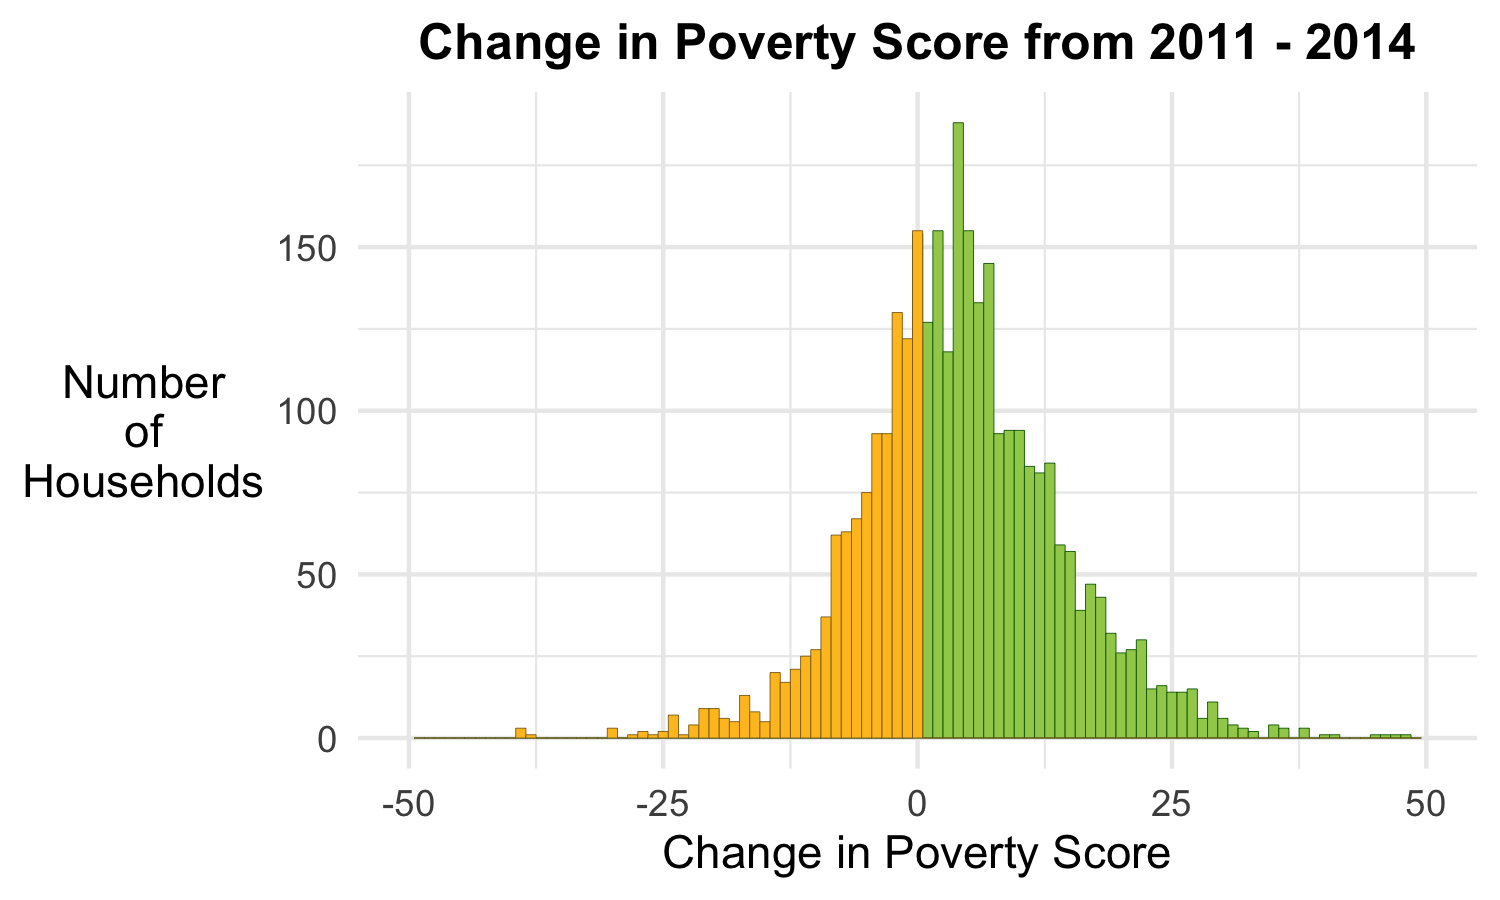
\includegraphics[width=.6\textwidth]{Figures/pscore_changes_r13.png}       
\end{figure}


\end{document}  